\section{Conference Funding}
\label{sec.fund}

Each student, whether self-funded or scholarship student, has a conference fund of 16,500 RMB. This can be used to reimburse registration fees, accommodation, transportation, and other expenses when attending conferences. If you don't use this money before graduation to \sout{go out and have fun around the conference} enrich your academic experience, it would be a waste. Although there's plenty of money, the application and reimbursement process is quite complicated. The main materials are:

\begin{itemize}
    \item e-bridge: \url{https://ebridge.xjtlu.edu.cn/}. After logging in, click on PGR Policies, Procedures and Forms to find the \textit{Postgraduate Research Students' Conference Fund Policy} and the \textit{Guideline and Procedures on Doctoral Student Travel Arrangement and Reimbursement}.
    \item Official flowchart
    \begin{figure}[H]
        \centering
        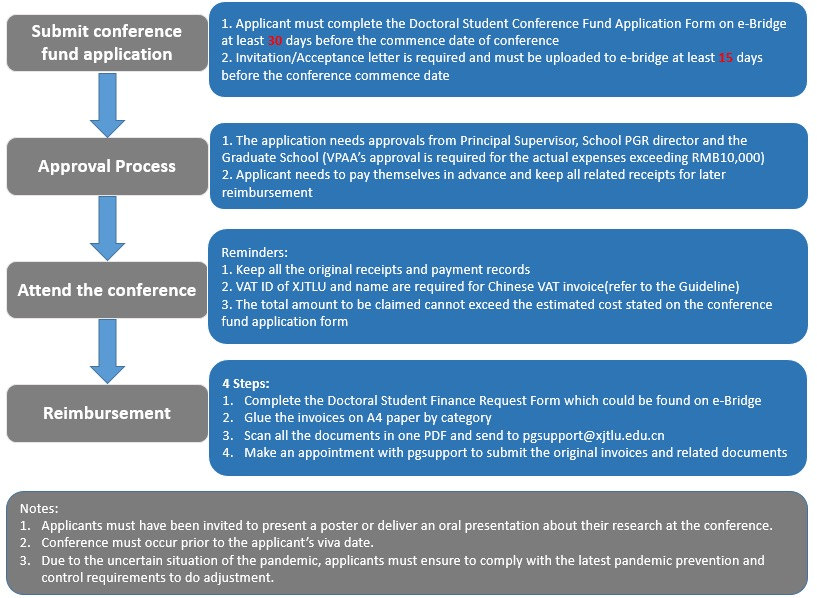
\includegraphics[width=0.9\columnwidth]{author-folder/Kai.Wu/fund-flowchart.jpg}
    \end{figure}
\end{itemize}

Please note:
\begin{enumerate}
    \item You must apply at least 30 days in advance. Therefore, it cannot be used for "a conference you suddenly heard about that's happening within 30 days."
    \item You must present at the conference; both poster or oral presentations are acceptable. Otherwise, you cannot use the funds.
    \item If you cannot use the university funds, you may be able to use some of your supervisor's funds. Due to the reasons above, I have used my supervisor's funds to reimburse several conferences. For details on how to proceed and whether your supervisor has such funds, please ask your supervisor.
\end{enumerate}

\begin{flushright}
(October 12, 2022 by \Wu) \\
(Translated by GPT)
\end{flushright}
